\documentclass[11pt]{texMemo-gibbons}
\usepackage[english]{babel}
\usepackage{siunitx}
\usepackage{graphicx}
\usepackage{blindtext}
\usepackage{amsmath,amssymb,units}
\usepackage[outdir=./]{epstopdf}
\memostudent{Ty Davis}
\memocourse{ECE 3210}
\memosubject{Lab 1, Lab Basics}
\memodate{\today}
\logo{
\includegraphics[width=0.5\textwidth]{ece_horiz.pdf}}

\begin{document}
\maketitle

\section{Introduction}
\label{sec:introduction}

This is the first lab of the semester in which we cover
the lab basics. We start by doing a brief analysis of
a simple RLC circuit (shown in Fig.~\ref{fig:circuit01}),
and then measuring and comparing the results of our
computation. Afterward, we practice some python by writing
an integral approximation function and comparing it
to an analytical solution of that integral.

\section{Theory}
\label{sec:theory}

\subsection{Circuit Analysis}
\label{sec:theory_circuit}

The RLC circuit that we analyzed in this lab is shown
in Fig.~\ref{fig:circuit01}. Using simple phasor analysis
we found that the magnitude of $y(t)$ is $72.056~\si{mV}$,
and the phase angle is $1.499~\si{rad}$ or $\ang{85.87}$.
Thus, $y(t)$ can be represented as the following. 

\begin{equation}
  \label{eq:y(t)}
  y(t)=0.072\cdot \sin (2\pi \cdot 10000 t + 1.499)
\end{equation}

\subsection{Computation}
\label{sec:theory_computation}

Equation 2.1 given in the Lab Manual is shown below.

\begin{equation}
  \label{eq:analytical}
  y(t)=\int^t_{-\infty}5e^{-\tau}u(\tau)d\tau
\end{equation}

The integral can be simplified to the following:

\[ y(t)=5 \cdot \int^t_{0}e^{-\tau}d\tau \]

And this equates to 
\begin{equation}
  y(t) = 
  \begin{cases}
    -5e^{-t}+5 & t \geq 0 \\
    0 & \text{otherwise}
  \end{cases}
  \label{eq:solution}
\end{equation}


As will be shown later in the report, this analytical
solution will be compared against the py\_cumtrapz function
we've written in python which approximates integrals
by summing trapezoids.

\section{Results}
\label{sec:results}

\subsection{Circuit Analysis}

The purpose of the lab was mostly to remind ourselves
with how to use the lab equipment and familiarize ourselves
with the techniques we will employ in later labs. After
a brief analysis of the circuit in Fig.~\ref{fig:circuit01},
we plotted the expected input and output, and compared
to the measured values we grabbed from the oscilloscope
when we built and measured the circuit. Refer to Fig.~\ref{fig:plots01}.

Then we practiced gathering the data from a frequency sweep of the
oscilloscope. The results can be found in Fig.~\ref{fig:bode_plots}.

\subsection{Computation}

In the computation section of the lab we plot the results
of our analytical solution shown in Eq.~\ref{eq:solution}
against the approximation we achieved from our py\_cumtrapz
function. The results can be found in Fig.~\ref{fig:comparison}.


\section{Discussion and Conclusions}
\label{sec:conclusions}

As can be seen in Fig.~\ref{fig:plots01}, the observed
values follow very close to the analysis that was calculated.
The observed output values especially lined up right
with the analytical solution given in Eq.~\ref{eq:y(t)}.
The result of the phasor circuit is another sine wave
that has a decreased magnitude (down to just 72 mV from
the 1 V input wave), and it is $\sim\ang{85}$ ahead
of the input signal. These numbers line up great with the 
values shown in the Bode plots from Fig.~\ref{fig:bode_plots}, where
the magnitude of the signal is somewhere around -22 dB and the phase
is just shy of $\ang{90}$.

In the computation portion of the lab, we compared our
py\_cumtrapz function (which approximates the integral
of any function) against the analytical solution we
found in Eq.~\ref{eq:solution}. We made the comparison
over the range $t \in [-1,5]$. The results from Fig.~\ref{fig:comparison}
show that our implementation of the py\_cumtrapz function
and the analytical solution are nearly identical, certainly within
the tolerance of an approximation that uses only 70 points within
the range for a calculation. Separating the range into more subdivisions
would certainly yield a more accurate result.

\clearpage

\begin{figure}[h!]
  \centering
  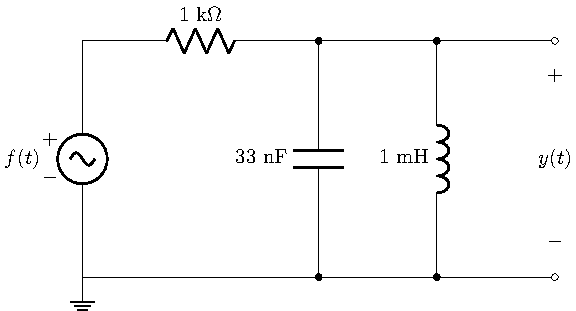
\includegraphics{circuits/circuit_01.pdf}
  \caption{Circuit for analysis in the lab.}
  \label{fig:circuit01}
\end{figure}

\begin{figure}[h!]
  \centering
  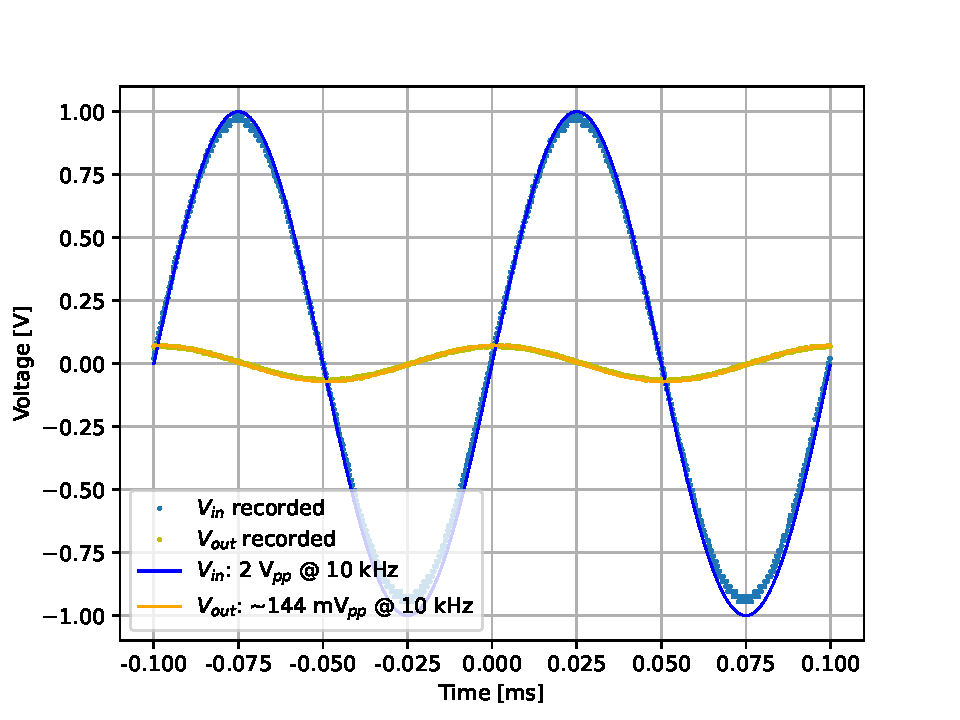
\includegraphics[width=0.7\textwidth]{plots/circuit_analysis.pdf}
  \caption{Plot for the circuit analyzed in Fig.~\ref{fig:circuit01}.}
  \label{fig:plots01}
\end{figure}

\begin{figure}[h!]
  \centering
  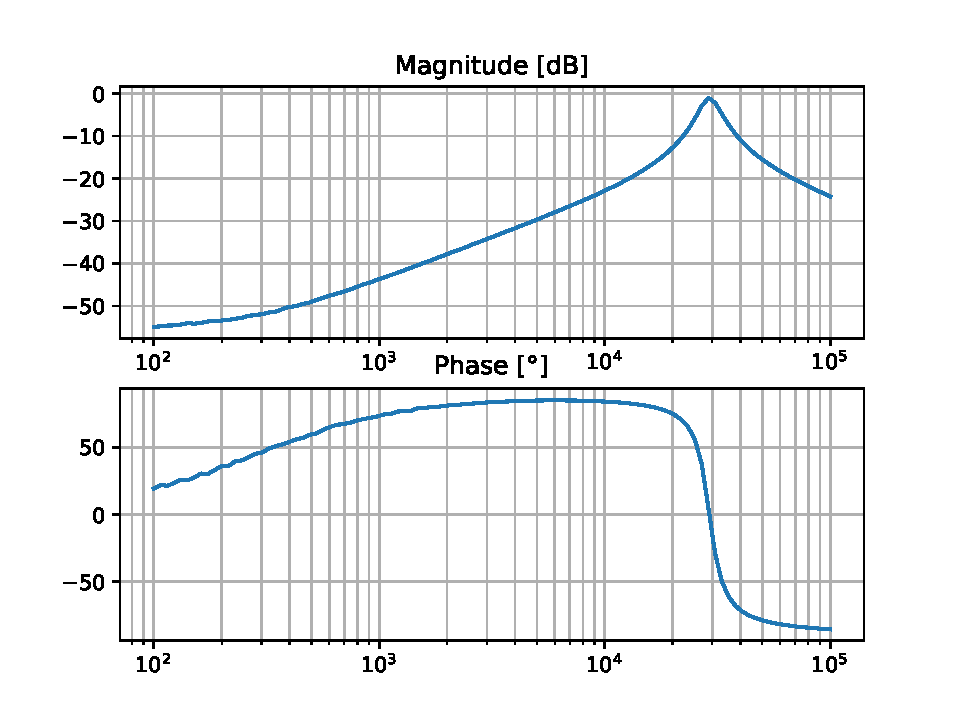
\includegraphics[width=0.7\textwidth]{plots/bode_plots.pdf}
  \caption{Bode plot of the frequency analysis for the circuit in Fig.~\ref{fig:circuit01}.}
  \label{fig:bode_plots}
\end{figure}

\begin{figure}[h!]
  \centering
  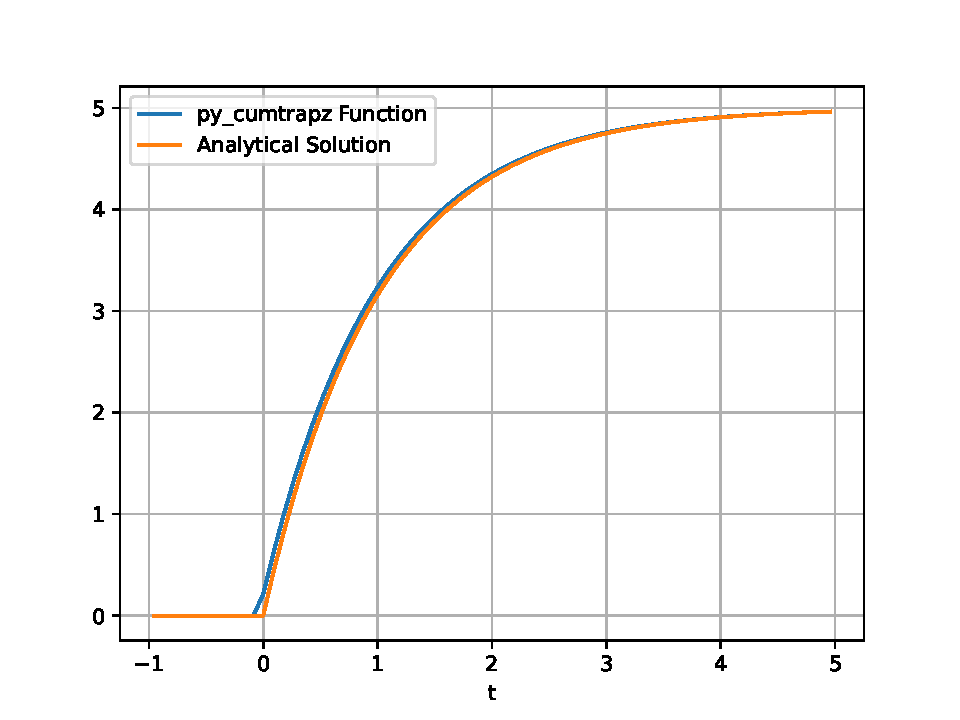
\includegraphics[width=0.7\textwidth]{plots/comparison.pdf}
  \caption{Comparison of the py\_cumtrapz function and the analytical solution.}
  \label{fig:comparison}
\end{figure}


\end{document}
%%% Local Variables:
%%% mode: latex
%%% TeX-master: t
%%% End:
